%******************************************************************************%
%                                                                              %
%                 nanotekspice/tex for Epitech's C++ Knowledge Unit            %
%                 Made by: Jason Brillante                                     %
%                                                                              %
%******************************************************************************%



\documentclass{koala-en}

\lstdefinelanguage{Avm}
{
  backgroundcolor=\color{gray!15},
  basicstyle=\scriptsize\ttfamily,
  breaklines=true,
  columns=fullflexible,
  frame=lines,
  tabsize=4,
  numbers=left,
  numberstyle=\scriptsize\ttfamily,
  numbersep=5pt,
  showspaces=false,
  showstringspaces=false,
  showtabs=false,
  breaklines=true,
  commentstyle=\color{nicerred},
  morecomment=[l]{;},
  keywordstyle=\color{nicerblue}\ttfamily,
  morekeywords={push, pop, dump, assert, add, mul, sub, div, mod, print, exit},
}

\lstset{language=Avm}

%******************************************************************************%
%                                                                              %
%                                Prologue                                      %
%                                                                              %
%******************************************************************************%

\begin{document}

\title{\textbf{Project C++}}
\subtitle{\textbf{NanoTekSpice}}
\member{Koalab}{koala@epitech.eu}
%\member{Jason Brillante}{brilla_a@epitech.net}

\summary
{
  The purpose of this project is to create a digital electronic simulator.
}

\maketitle

\tableofcontents

\renewcommand{\labelitemi}{$\bullet$}
\renewcommand{\labelitemii}{$\circ$}


%******************************************************************************%
%                                                                              %
%                            I - Digital Electronic                            %
%                                                                              %
%******************************************************************************%
\chapter{Digital Electronic}

        There is variety of programming languages, C, Lisp, Basic, APL, Intercal...
They all have their specificities and may be efficient in different ways.
They mainly rely on a compiler to work. This compiler will transform
the code which is written in almost human language to a more primitive form.\\

This primitive form is the assembly language if seen as its human readable form,
or machine language if seen as the microprocessor sees it.\\

The same way there is a variety of programming languages, there is a lot of
assembly languages: at least one per processor family, sometimes one per processor,
sometimes several per processor.\\

Of course, knowing an assembly language for a microprocessor may not be enough
to be efficient: a microprocessor is not a full machine. You may need to know
how your machine works in order to create a usefull program in assembly:
Which address for the graphic card? Which trap for this system call?\\

Under assembly languages and machine languages, there is the hardware itself.
The hardware is built with digital electronic components: chipsets.
Chipsets are tiny little functions with inputs and outputs that can
be linked together to create more powerful functions, exactly like with
software functions.\\

These functions are exclusively based on boolean logic. So it only gets
and returns true or false values. In this project, you will have to create a
graph. In this graph, nodes will be simulated digital electronic components,
inputs or outputs.\\

What does a chipset look like? Here is one:

  \begin{center}
    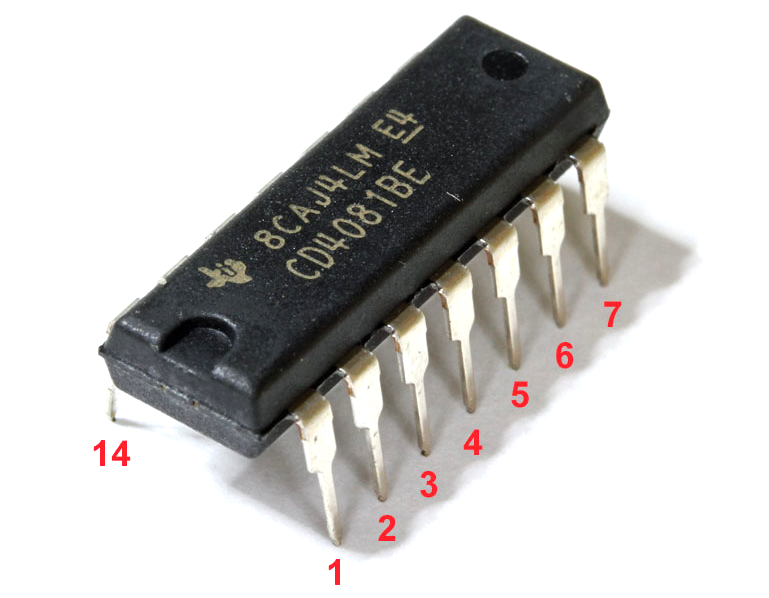
\includegraphics[height=3cm]{chipset.png}
  \end{center}


%******************************************************************************%
%                                                                              %
%                            II - Architecture                                 %
%                                                                              %
%******************************************************************************%
\chapter{Chipset}

  Here is an example of what's inside a simple chipsets: the 4081.

  \begin{center}
    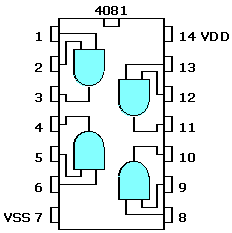
\includegraphics[height=5cm]{4081.png}
  \end{center}

  The 4081 is a little box that contains four AND gates. An AND gate has
  two inputs (A and B) and one output (S). The 4081 features 14 connectors.
  
  \begin{itemize}
    \item Pin 1 and pin 2 are inputs of one of the and gate, let's say gate 1.
    \item Pin 3 is the output of gate 1.
    \item Pin 4 is the output of gate 2.
    \item Pin 5 and 6 are input of the gate 2.
    \item Pin 7 (VSS) is here for electrical purpose. We will ignore it in this project.
    \item Pin 8 and 9 are inputs of gate 3.
    \item Pin 10 is the output of gate 3.
    \item Pin 11 is the output of gate 4.
    \item Pin 12 and 13 are inputs of gate 4.
    \item Pin 14 (VDD) is here for electrical purpose. We will ignore it in this project.
  \end{itemize}
  
  Here is the AND gate ``truth table'':

  \begin{center}
    \begin{tabular}{ccc}
      A & B & S\\
      0 & 0 & 0\\
      0 & 1 & 0\\
      1 & 0 & 0\\
      1 & 1 & 1\\
    \end{tabular}
  \end{center}

  Note that this is absolutely equivalent to the following function:\\
  \lstset
    {
      language=C++,
      morekeywords=[2]{IComponent}
      morekeywords=[3]{rhs}
      keywordstyle=[2]\color{nicergreen}\ttfamily,
      keywordstyle=[2]\color{nicerorange}\ttfamily,
      stringstyle=\color{nicergreen}\ttfamily
    }
  \lstinputlisting[language=C++]{./and_gate.c}
    
  There is plenty of chipsets. Some of them are primitive, like the 4081,
  some others bring more complicated functions like counting or serialising
  functions. Microprocessors are one of the more complicated family of chipset
  existing by providing interpreters.\\

  Of course, microprocessors are built with more simple chip, which happened
  to be built from components like the 4081 chipset. Everything can be reduced
  to boolean logic.\\

%******************************************************************************%
%                                                                              %
%                            III - The Undefined State                         %
%                                                                              %
%******************************************************************************%
\chapter{The Undefined State}

The boolean algebra is composed of only two states: true and false. In the
electronic world, true means VCC volt. VCC is the alimentation of the system.
In a lot of case, VCC is 5 volt. In the electronic world, false means, in
most cases, 0 volts.\\

It creates a problem we won't treat here: there is a lot of value under 0 and
a lot above 5, and even an infinite between 0 and 5.\\

It also creates another problem we will have to treat:
What if a component A needs to know the value S to compute its output, but S
needs its output to be defined?\\

The answer cannot be true or false. The answer is that the value is undefined, a
third state. So you will not compute pure boolean algebgra. You will have to
integrate an undefined state.\\

Get out bool! Welcome enum!

%******************************************************************************%
%                                                                              %
%                            IV - The project                                  %
%                                                                              %
%******************************************************************************%
\chapter{The project}

NanoTekSpice is a logic simulator that is able to build a graph thanks to a
configuration file, as well as inject values inside the graph to get results.

\section{The configuration file}

    \subsection{Example}

    Here is an example of configuration file. It contains a graph description.

    \lstinputlisting[language={}]{./_3input_and_gate.nts}

    \subsection{Description}

    The first part, which starts with the ``.chipsets:'' statement allows you
    to declare components that will be used by the program and name them.
    Some components may need a value. This value will be passed right after
    the name between parenthesis.\\

    The second part, which starts with the ``.links:'' statement allows you
    to declare links between components. You have to precise which component
    you wish to link and which pin.\\

    Space between keywords on the same line may be spaces or tabs. Newline
    terminates the statement.\\

    Comments start with a '\#' and finish with a newline. A comment can
    be either at the start of a line, or after an instruction.\\

    Here are a few special components:
    
  \begin{itemize}

    \item \textbf{input} : Creates a value directly linked to the command line.
      The value may be 0 or 1 and must be given this way:
      ./nanotekspice circuit\_file.ts input\_name=input\_value

    \item \textbf{clock} : Creates an input that works the same way as \textbf{input}
      except that its value is inverted after each simulation.

    \item \textbf{true} : This component have one pin that is always true.

    \item \textbf{false} : This component have one pin that is always false.
      
    \item \textbf{output} : Creates an output that writes its state on stdout at the end of
      each simulation. If there are several outputs, they must be
      ascii sorted.

  \end{itemize}

\subsection{Errors}

    When one of the following cases happens, NanoTekSpice must raise an 
  exception and stop the execution of the program neatly. It is forbidden
  to raise scalar exceptions. Moreover, exception classes must inherit from 
  \verb=std::exception= of the \texttt{STL}.

  \begin{itemize}
    \item The circuit file includes one or several lexical errors
      or syntactic errors.
    \item A component type is unknown
    \item A component name is unknown
    \item The given pin does not exist
    \item Several components share the same name
    \item Not every output is linked
    \item Missing input value on command line
    \item Unknown input specified by command line
    \item No chipset section
    \item No links section
  \end{itemize}

    Perhaps there are others errors. However, your simulator
   must never crash! (segfault, bus error, infinite loop ...)

   \subsection{Execution}
   
   Your simulator must be able to run with a circuit file and inputs value passed as parameter.
   The simulator also reads on stdin a few commands:
   
   \begin{itemize}
    \item \textbf{exit} : It closes the program.
    \item \textbf{display} : It prints on stdout the value of all outputs sorted by name.
    \item \textbf{input=value} : It changes the value of an input. (Not a clock)
    \item \textbf{simulate} : It launches a simulation.
    \item \textbf{loop} : Simulate without prompting again until SIGINT.
    \item \textbf{dump} : Call the Dump method of every IComponent
  \end{itemize}

  Your simulator must launch one simulation directly after being launched, then display.
  Your simulator must handle CTRL+D correctly.\\
  
  Now let's see some examples of execution.

  \begin{lstlisting}
    cat -e or_gate.nts
    .chipsets:
    input a
    input b
    4071 or
    output s
    .links:
    a:1 or:1
    b:1 or:2
    or:3 s:1
    ./nanotekspice or_gate.nts a=0 b=0
    s=0
    > a=1
    > simulate
    > display
    s=1
    > exit
    C:\>
  \end{lstlisting}

  \begin{lstlisting}
    C:\> cat -e bad.nts
    .chipsets:
    input i
    output o
    .links:
    C:\> ./nanotekspice bad.nts i=0
    Output 'o' is not linked to anything.
    C:\>
  \end{lstlisting}

  \hint
  {
      The error message is given as an example. Feel free to use yours instead.
  }

  \section{The parser}

    This project is probably your first try at parsing a configuration file. Thus, we will guide you through
  parsing steps.
  Here is the interface your parser must implement.

  \lstinputlisting[language={C++}]{./IParser.hpp}

    The idea behind this parser is the same as presented by Victor Boudon in his slides about the 42sh parser
  (they will be given as annexes).

  \begin{itemize}
  \item \textbf{ASTNodeType} : The type of a node in the tree.
  \item \textbf{s\_ast\_node} : A node of the output tree.
  \item \textbf{Parser} : The actual interface.
    \begin{itemize}
    \item \textbf{feed(std\:\:string const\&)} : Appends the string to the current input.
    \item \textbf{parseTree(t\_ast\_node\&)} : Takes the AST root and goes through the whole tree.
    \item \textbf{createTree()} : Parses the input string to produce the ouput tree.
    \end{itemize}
  \end{itemize}

    From this interface, one could wonder how to achieve a correct complete parser. Well, it is not that hard.
  You have to split the parsing in two steps : build the AST (Abstract Syntax Tree), then actually go through this tree, calling
  a function depending on the type of each node.
  As you might have understood from Victor's example, you will have to write / design your own grammar, which you will use to implement your parser.
  You will also have to write your own semantic actions, which are the functions associated with each one of the operators in your grammar. For example,
  imagine the grammar of a calculator, 'add' is a semantic action -> from a character ('+'), you extract a semantic meaning (the addition of two operands),
  and apply it.

  \hint
      {
          The whole point of this exercise is to give you a basic understanding of what is a good parser. For reference, this is called a Recursive Descent Parser.
        Feel free to read anything you'd like about this kind of parsers, but be careful, you have to respect our interface.
      }


%******************************************************************************%
%                                                                              %
%                       V - Technical considerations                           %
%                                                                              %
%******************************************************************************%
\chapter{Technical considerations}

    In order to help you with your code, we give you the following instructions that 
  you have to respect. For each instruction, you must understand why this particular
  one is imposed. We are not providing these instructions randomly or to bore you to 
  death!

\section{The IComponent interface}

     Each of your component classes MUST implement the following IComponent interface:

  \lstset
      {
        language=C++,
        morekeywords=[2]{IComponent}
        morekeywords=[3]{rhs}
        keywordstyle=[2]\color{nicergreen}\ttfamily,
        keywordstyle=[2]\color{nicerorange}\ttfamily,
        stringstyle=\color{nicergreen}\ttfamily
      }
    \lstinputlisting[language=C++]{./IComponent.hpp}

    Component classes implementing the IComponent interface are the following ones.
    You can find manuals about these components in the same directory you found
    this subject.\\

  \begin{itemize}
    \item \textbf{4001} : Four NOR gates.
    \item \textbf{4008} : 4bits adder.
    \item \textbf{4011} : Four NAND gates.
    \item \textbf{4013} : Dual Flip Flop.
    \item \textbf{4017} : 10bits Johnson decade.
    \item \textbf{4030} : Four XOR gates.
    \item \textbf{4040} : 12 bits counter.
    \item \textbf{4069} : Six INVERTER gates.
    \item \textbf{4071} : Four OR gates.
    \item \textbf{4081} : Four AND gates.
    \item \textbf{4094} : 8bits shift register.
    \item \textbf{4514} : 4bits decoder.
    \item \textbf{4801} : Random access memory.
    \item \textbf{2716} : Read only memory. 2716 must takes a value
      when declared. In the .chipsets: section,  you must
      precise a file that will contain the data written in the ROM:
      2716      rom(cp\_m.dat)
  \end{itemize}

  \warn
  {
	  \textbf{Important} : It is FORBIDDEN to manipulate pointers or
	  references on each of these classes in your graph. You are allowed to manipulate
          pointers ONLY on IComponent.
  }

\section{Creation of a new IComponent}

    You have to write a member function of a class \textbf{relevant} to your
  system that will allow you to create new components in a generic way. This
  function must have the following prototype:

  \begin{lstlisting}
    IComponent * createComponent(const std::string &type, const std::string &value);
  \end{lstlisting}

    Depending on the value of the string passed as a parameter, the member function
  \texttt{createComponent} creates a new \texttt{IComponent} by calling  one of the
  following \texttt{private} member function:

  \begin{lstlisting}
    IComponent * create4001(const std::string &value) const;
    IComponent * create4013(const std::string &value) const;
    IComponent * create4040(const std::string &value) const;
    // Etc...
  \end{lstlisting}

    In order to choose the right member function for the creation of the new
    \texttt{IComponent}, you MUST create and use an array (here, \texttt{vector}
    shows little interest) of pointers to member functions.

%******************************************************************************%
%                                                                              %
%                               VI - Boni                                      %
%                                                                              %
%******************************************************************************%
\chapter{Bonus}

There is several bonuses available. Here are a few example:

\begin{itemize}
    
  \item Terminal output component. Takes 8 bits as ascii code, and 1 bit
    which prints the character on stderr while switching from 0 to 1.

  \item Graphic output of the graph. (Feel free to add a .graphic: section
    inside your configuration file with graphics information.
    
  \item Graphic component ``7seg'':
    Takes 4 bits as input. Display an hexadecimal number matching its entry.
    
  \item Graphic component ``matrix'':
    Takes 8 bits as a color shade and takes 12 bits as pixel select.
    Output is a 64*64 pixels picture.
    
  \item i4004 support (Or any other microprocessor, even your own creation.
    Must be turing complete).

  \item Simulating a little computer.
    
\end{itemize}

Feel free to use SFML, SDL, Allegro, mlx or lapin for graphics.
\textbf{For graphics only.}

%******************************************************************************%
%                                                                              %
%                               VII - Instructions                             %
%                                                                              %
%******************************************************************************%
\chapter{Instructions}

    You are more or less free to implement your machine how ever you want.
  However there are certain rules:

  \begin{itemize}

    \item Your program name must be ``nanotekspice''.

    \item You must provide a static library ``libnanotekspice.a'' containing
      all your functions except the main function. This library will be used
      to test your IComponent system.
    
    \item All libraries except for \texttt{STL} are strictly
	prohibited. Graphic library can be used under bonus condition.

    \item You must use \texttt{STL} as much as you can. Your project must
      contains at least one container and one exception class from \texttt{STL}. 
     The use of at least one algorithm from \texttt{STL} will be appreciated. 
     Be very careful!

    \item The only functions of the \texttt{libc} that are authorized are those one
      that encapsulate system calls, and that don't have a C++ equivalent.

    \item ``split'', ``strtowordtab'', and so on must \textbf{not} be
      used for parsing.

    \item Each value passed by copy instead of reference or by
          pointer must be justified. Otherwise, you'll loose points.

    \item Each non \texttt{const} passed as parameter must be
      justified. Otherwise, you'll loose points.

    \item Each member function or method that does not modify the current
      instance and which is not \texttt{const} must be justified. Otherwise, 
      you'll loose points.

    \item There are no \texttt{C++} norm. However if a code is reckoned
      to be unreadable or dirty, this code will be penalized. Be
      serious please!

    \item Keep an eye on this project instructions. It can change with time!

  \end{itemize}


%******************************************************************************%
%                                                                              %
%                          VIII - Turn in instructions                         %
%                                                                              %
%******************************************************************************%
\chapter{Turn in instructions}

    You must turn in you project in the repository provided by
  Epitech.\\
    The repository name is cpp\_nanotekspice.\\

    Repository will be cloned at the exact hour of the end of the project, 
    intranet \texttt{Epitech} being the reference.\\

   Only the code from your repository will be graded during the oral defense.\\

   Good luck!


%******************************************************************************%
\end{document}
